\documentclass[letterpaper,12pt,fleqn]{article}
\usepackage{matharticle}
\usepackage{tikz}
\pagestyle{empty}
\newcommand{\floor}[1]{\left\lfloor#1\right\rfloor}
\begin{document}
\section*{Division Algorithm}

\begin{theorem}
  Let $m,n\in\Z$ and $n>=0$. There exists unique integers $q$ and $r$ such that:
  \[m=qn+r\]
  where $0\le r<n$.

  $q$ is called the \emph{quotient} and $r$ is called the \emph{remainder}.
  
  $m$ is called the \emph{dividend} and $n$ is called the \emph{divisor}.
\end{theorem}

This can be demonstrated graphically by partitioning the real number line into
segments of length $n$ and then placing $m$ on the line:

\bigskip

\begin{center}
  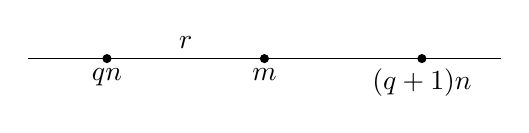
\begin{tikzpicture}
    \draw (0,0) -- (6,0);
    \draw [fill=black] (1,0) circle [radius=0.05];
    \draw [fill=black] (3,0) circle [radius=0.05];
    \draw [fill=black] (5,0) circle [radius=0.05];
    \node [below] at (1,0) {$qn$};
    \node [below] at (3,0) {$m$};
    \node [below] at (5,0) {$(q+1)n$};
    \node [above] at (2,0) {$r$};
  \end{tikzpicture}
\end{center}

\begin{theproof}
  Let $S=\{m-kn\mid k\in\Z\}$ \\
  Let $T=\{s\in S\mid s\ge0\}$ \\
  Note that $T\ne\emptyset$, since $m>=kn$ for some suitable $k\le0$ \\
  Thus, by the well-ordering principle, $T$ has a minimum \\
  Let $r=m-qn$ be that minimum for some $q\in\Z$ \\
  By construction, $r>0$ \\
  ABC: $r\ge n$ \\
  $r>r-n\ge0$ \\
  $r>(m-qn)-n\ge0$ \\
  $r>m-(q+1)n=ge0$ \\
  But $m-(q+1)n\in T$ \\
  CONTRADICTION (of the minimality of $r$)! \\
  $\therefore m=qn+r$ and $0\le r<n$ \\

  Now, assume $m=q_1n+r_1$ and $m=q_2n+r_2$ with $0\le r_1,r_2<n$ \\
  $q_1n+r_1=q_2n+r_2$ \\
  $(q_1-q_2)n=(r_2-r_1)$ \\
  $0\le r_1<n$ \\
  $-n<-r_1\le0$ \\
  $0\le r_2<n$ \\
  $-n<r_2-r_1<n$ \\
  $-n<(q_1-q_2)n<n$ \\
  $-1<q_1-q_2<1$ \\
  But, by closure, $q_1-q_2\in\Z$ \\
  So $q_1-q_2=0$ \\
  $\therefore q_1=q_2=q$ \\
  $0n=r_2-r_1=0$ \\
  $\therefore r_1=r_2=r$ \\

  $\therefore$ there exists unique $q,r\in\Z$ such that $m=qn+r$ and
  $0\le r<n$.
\end{theproof}

Given $m$ and $n$, the greatest integer function can be used to calculate
$q$ and $r$:
\[q=\floor{\frac{m}{n}}\]
\[r=m-nq\]

\begin{example}
  Let $m=123$ and $n=10$:
  \[q=\floor{\frac{123}{10}}=12\]
  \[r=123-12\cdot10=123-120=3\]
  \[123=12\cdot10+3\]
  \[0\le3<10\]

  Let $m=-123$ and $n=10$:
  \[q=\floor{\frac{-123}{10}}=-13\]
  \[r=-123-(-13)\cdot10=-123+130=7\]
  \[-123=-13\cdot10+7\]
  \[0\le7<10\]
\end{example}

\end{document}
